\subsubsection{Cosine Similarity}

The topics clustering helps the cosine based distance. It seems that splitting articles into topics makes a better contrast between years. This result can be well interpreted. Indeed, because the years are represented by vectors containing the frequencies of words. The dimension of these vectors are reduced which is a consequence of that a word belongs to a specific topic. Therefore the angle between them is big and due to the language itself over time and not over a topic. 

\begin{figure}[H]
    \begin{minipage}[b]{0.48\linewidth}
        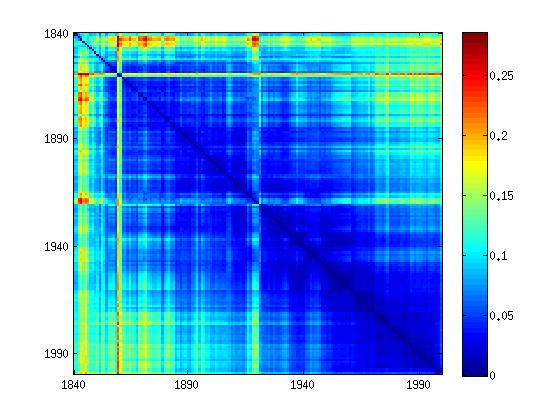
\includegraphics[scale=0.3]{Pictures/topics/cos/topic1.jpg}
        \caption{Cosine distance on "Religion" topic}
        \label{cos_topic1}
    \end{minipage}\hfill
    \begin{minipage}[b]{0.5\linewidth}
        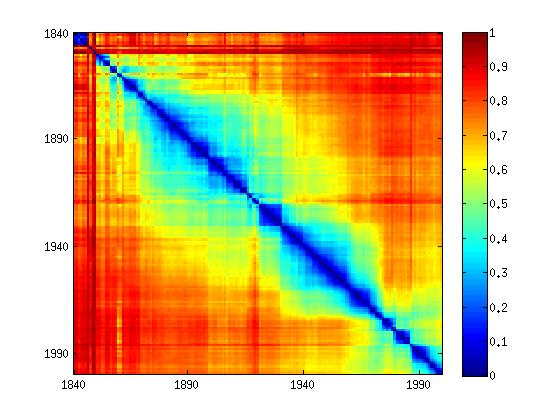
\includegraphics[scale=0.3]{Pictures/topics/cos/topic3.jpg}
        \caption{Cosine distance on "Undefined" topic}
        \label{cos_topic3}
    \end{minipage}\hfill
\end{figure}

There is some topics where we cannot distinguish any drift where an example is shown in figure \ref{cos_topic1}. The concerned topic is about history and religion, so it seems that it doesn't change over years and the language drift is hard to enhance for that kind of subject. On the contrary, there is some topics where a drift over years is well marked such as in figure \ref{cos_topic3}. For those cases, the fact that the articles are separated in topics gives an improvement for the cosine metric.

\begin{figure}[H]
    \begin{minipage}[b]{0.48\linewidth}
        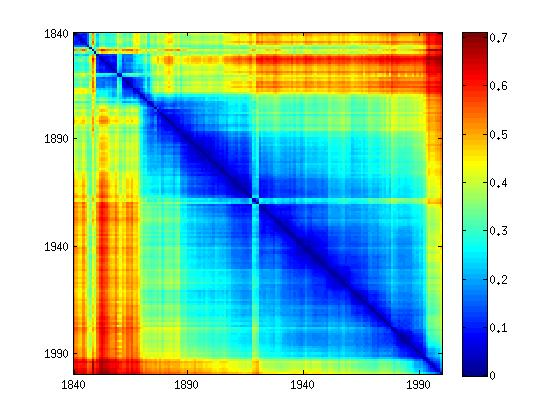
\includegraphics[scale=0.3]{Pictures/topics/cos/topic7.jpg}
        \caption{cosine distance on "Swiss politics" topic}
        \label{cos_topic7}
    \end{minipage}\hfill
    \begin{minipage}[b]{0.5\linewidth}
        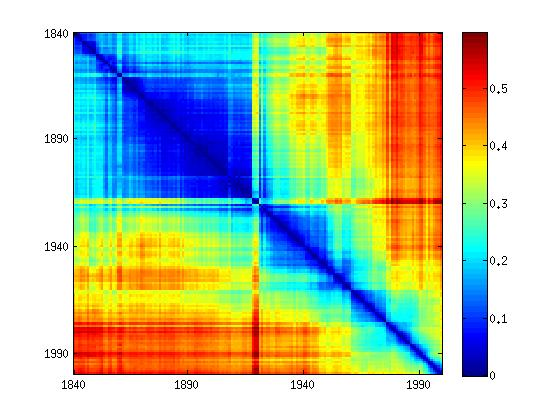
\includegraphics[scale=0.3]{Pictures/topics/cos/topic9.jpg}
        \caption{cosine distance on "Theatre and Music" topic}
        \label{cos_topic9}
    \end{minipage}\hfill
\end{figure}

We have also interesting topics such as Swiss politics or music in figures \ref{cos_topic7} and \ref{cos_topic9} where a drift is also enhanced compared to the distance on the whole corpus but the changes are not proportional along the time. This can suggest that there is a kind of acceleration or deceleration over time in some specific topics.